\documentclass{article}

\usepackage{tikz}
\usetikzlibrary{shapes}

\usepackage{dirtree}
\usepackage{hyperref}
\usepackage{listings}
\usepackage{color}


\definecolor{codegreen}{rgb}{0,0.6,0}
\definecolor{codegray}{rgb}{0.5,0.5,0.5}
\definecolor{codepurple}{rgb}{0.58,0,0.82}
\definecolor{backcolour}{rgb}{0.95,0.95,0.92}
\definecolor{keywordcolour}{rgb}{0.0,0.0,0.92}
 
\lstdefinestyle{mystyle}{
    backgroundcolor=\color{backcolour},   
    commentstyle=\color{codegreen},
    keywordstyle=\color{keywordcolour},
    numberstyle=\tiny\color{codegray},
    stringstyle=\color{codepurple},
    basicstyle=\footnotesize,
    breakatwhitespace=false,         
    breaklines=true,                 
    captionpos=b,                    
    keepspaces=true,                 
    numbers=left,                    
    numbersep=5pt,                  
    showspaces=false,                
    showstringspaces=false,
    showtabs=false,                  
    tabsize=2
}

Server Side Frontend Code.



\lstset{style=mystyle}

\author{Marco Jakob}
\title{Kubernetes Full Stack Application}

\begin{document}

\maketitle
\newpage
\tableofcontents
\newpage

\section{Introduction}
This Introduction should give an end to end overview to deploy a sample Application with multiple Services and a Databases completely on Kubernetes.
The Application generates Random Numbers, saves them with a Timestamp on a database. Displays the new Number on a Frontend and also shows Graphs from previous Random Numbers based on their Producers Id.
The Goal of the whole application is first to create an end to end Application fully Cloud native which runs as well locally without any changes. The second goal is to show graphically the self healing process of Kubernetes, namely when we delete a random generator Pod, it should automatically create a new Random generator Pod with a new Id.
\section{Prerequisites}
To create the application it is assumed that we already have a machine with the following Software running:
\begin{itemize}
\item Java Development Kit (minimum 1.8)
\item Maven build tool
\item Python 3.6
\item Docker
\item Angular (minimum version 6) with the ng command
\end{itemize}
\subsection{Technology}
\begin{table}[h]
\begin{tabular}{ll}
\textbf{Service} & \textbf{Technology}  \\ \hline
Random Number Generator circle& Python Flask \\
Database to store previous Numbers & Mysql Database \\
Microservice for requesting new Numbers & Spring Boot Java \\
Microservice for gathering Statistics & Spring Boot Java \\
Frontend & Angular with Spring Boot \\
Routing Server & Nginx \\
Server OS & Ubuntu Server 18.5.1  LTS
\end{tabular}
\end{table}

All the Applications are Running inside of an own Docker Container and Managed within a Kubernetes Pod and accessible via a Kubernetes Service where only the Frontend Service is bound to a Node Port.
\subsection{Model}
The Following Picture should give an overview about the different Services and how they work with each other.

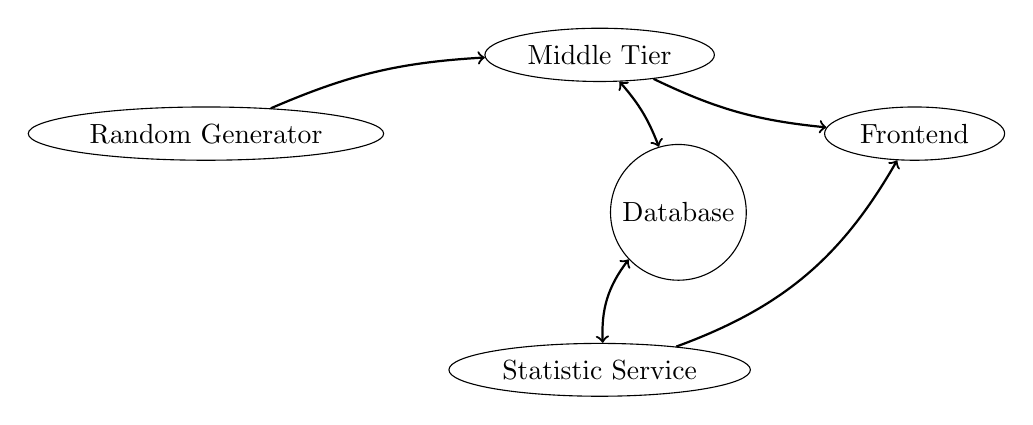
\begin{tikzpicture}
\node (A) at (0,0) [ellipse, draw] {Random Generator};
\node (B) at (5,-3) [ellipse, draw] {Statistic Service};
\node (C) at (6,-1) [circle, draw] {Database};
\node (D) at (9,0) [ellipse, draw] {Frontend};
\node (E) at (5,1) [ellipse, draw] {Middle Tier};

\draw[<->, thick] (B) to[bend left=20] (C);
\draw[->, thick] (B) to[bend right=20] (D);
\draw[->, thick] (A) to[bend left=10] (E);
\draw[->, thick] (E) to[bend right=10] (D); 
\draw[<->, thick] (E) to[bend left=10] (C);

\end{tikzpicture}



\section{Create Services}
\subsection{Database}
In the further sections we will use a plain mysql docker container as a database. In order to use the Application completely locally, a local mySQL database has to be installed and a schema for the random generator application needs to be provided for a specific randgenuser.
If there is not yet a local mySQL database installed it can be done with the following command:
\begin{lstlisting}[language=Bash]
sudo apt-get update
sudo apt-get install mysql-server
\end{lstlisting}
After the installation log in to MySQL as root. 
\begin{lstlisting}[language=Bash]
sudo mysql
\end{lstlisting}
Now the Database and the user can be created and permissions to the respective schema will be given.
\begin{lstlisting}[language=SQL]
CREATE database db_example;
CREATE USER 'springuser'@'localhost' IDENTIFIED BY ThePassword;
GRANT ALL PRIVILEGES ON *.db_example TO 'springuser'@'localhost';
\end{lstlisting}
With this, the Database is ready to used by the Random Generator Example from localhost.

\subsection{Random Generator}
The Random Generator will be a verry simple Python App which has an unique Id per Service instance. It will return his id and a new Random Number. For this application we create a folder called RandGen with the following Structure.

\dirtree{%
.1 RandGen.
.2 Dockerfile.
.2 rand\_gen.py.
.2 requirements.txt.
}
The Dockerfile is needed to create the Docker Image which will be used from Kubernetes to Create the Random Generator Service.
rand\_gen.py is the complete Random Generator Python application based on Flask\footnote{More information about Flask can be found on the official Homepage \url{http://flask.pocoo.org/}}.
 \lstinputlisting[language=Python]{Applications/RandGen/rand_gen.py}
In requirements.txt are the Python packages specified. In this case it is flask. therefore this file contains only one line which is
\begin{verbatim}
Flask==1.0.2
\end{verbatim}

\subsection{Middle Tier}
The Middle Tier Application is created with Spring Initializer.
Unter the following link \url{https://start.spring.io/} Helps to bootstrap very fast a simple Spring Boot application.
In our case the fields should be filled out as followed:
\begin{tabbing}
\begin{tabular}{ll}
Project & Maven Project \\
Language & Java \\
Spring Boot & 2.1.3 (All versions would apply) \\
Group & ch.toky.randgen \\
Artifact & middletier \\
Name & MiddleTier \\
Description & Middle Tier Service for Random Generator Application \\
Packaging & Jar \\
Java Version & 8 \\
Dependencies & Web, JPA, MySQL, Rest Repositories
\end{tabular}
\end{tabbing}
The Website will create a zip file to download. This zipfile has to be extracted to the desired Project folder.
\dirtree{%
.1 middletier.
.2 Dockerfile.
.2 mvnw.
.2 mvnw.cmd.
.2 pom.xml.
.2 src.
}
all blue folders are already given. the Dockerfile still has to be created.

Now inside of the Project create the following Project Structure and files.

\dirtree{%
.1 ch.toky.randgen.middletier.
.2 MiddletierApplication.java.
.2 RandomNumber.java.
.2 ch.toky.rand-gen.middle-tier.model.
.3 PodStat.java.
.2 ch.toky.rand-gen.middle-tier.repository.
.3 PodStatRepository.java.
}
The file MiddleTierApplication.java should already be in place. as Spring Boot Initializr created this with the complete Folder structure. the packages controller, model and repository need to be created.
Inside of controller, A file named MiddletierController.java needs to be created with the following content.

Within the model package two new Files have to be created: PodStat.java and RandomNumber.java.

PodStat is an Entity and therefore the class has to be annotated with @Entity.
It contents the following fields with their respective getter and Setter Methods.
\begin{lstlisting}[language=Java]
@Id
@GeneratedValue(strategy=GenerationType.AUTO)
private Long podStatID;
private String id;
private Long timeStamp;
private Long counter;
\end{lstlisting}

The class RandomNumber is only a DTO which is retreived from the random generator Service. Therefore there is no need for a annotation.
Only the following Fields needs to be declared with their getters and setters:

\begin{lstlisting}[language=Java]
private String id;
private Long randNumber;
\end{lstlisting}

In the repository package the file PodStatRepository.java will be created.
As this java file is not a class but an interface it needs to be changed to interface and extends JpaRepository<PodStat, Long>
and it will be annotated with @Repository

Now those two methods are created 
\begin{lstlisting}[language=Java]
@Query("Select count(ps.id) from PodStat ps where ps.id = ?1")
Long countUniqueId(String id);

@Query("Select count(ps.id) from PodStat ps")
Long findMaxCount();
\end{lstlisting}

Witin the controller all the endpoints are declared. Therfore it will be annotaded with @RestController

Those fields are needed within the controller and are therefore declared first.
\begin{lstlisting}[language=Java]
@Autowired
private ObjectMapper objectMapper;
@Autowired
private PodStatRepository podStatRepository;
private Map<String, String> env = System.getenv();
\end{lstlisting}
As there should not be any hardcoded url according to the 12 Factor application \footnote{Accessible at \url{https://12factor.net/}}, the Url will be retreived through a System Variable.

Now a controller Method with the business logic can be declared:
\begin{lstlisting}[language=Java]
@RequestMapping(value = "/", produces = "application/json")
public RandomNumber getRandom() {

    RandomNumber randNum = getNewRandomNumber();
    Long maxCountId = podStatRepository.countUniqueId(randNum.getId());
    Long maxCountOverall = podStatRepository.findMaxCount();
    PodStat tmpPod = new PodStat();
    tmpPod.setId(randNum.getId());
    tmpPod.setTimeStamp(maxCountOverall+1);
    tmpPod.setCounter(maxCountId +1);
    podStatRepository.save(tmpPod);

    return randNum;

}
\end{lstlisting}
The above Method listens on the path / and returns the Random number after saving it to the database with the actual count.

Now the last Method is used to retreive the Random Number from the Random Generator Service.
\begin{lstlisting}[language=Java]
private RandomNumber getNewRandomNumber() {

    String randGenUrl=env.get("RANDOM_GENERATOR_URL");
    String URL = randGenUrl;
    RestTemplate restTemplate = new RestTemplate();

    return   restTemplate.getForObject(URL, RandomNumber.class);

}
\end{lstlisting}
Above Source code contains the Controller and the Service, which should be separated optimally.
Next two files represents POJOs which are going to be used from controller and provided by Repositories.

The last thing which needs to be done for the Middle Tier Service is to setup the default values for the Database Connection.
\begin{lstlisting}[language=Properties]
spring.jpa.hibernate.ddl-auto=update
spring.datasource.username=random_user
spring.datasource.password=random_password
spring.datasource.url=jdbc:mysql://localhost:3306/rand_numbers
\end{lstlisting}
The datasource configurations are going to be overwritten by Environment Variables once they run inside of a Docker Container.



\subsection{Statistic Service}
The Statistic Service has the same setup as the Middle Tier client.
Therefore the Project will be created too with Spring Boot initializer.
\begin{tabbing}
\begin{tabular}{ll}
Project & Maven Project \\
Language & Java \\
Spring Boot & 2.1.3 (All versions would apply) \\
Group & ch.toky.randgen \\
Artifact & stattier \\
Name & Stattier \\
Description & Statistic Tier Client for Random Generator Application \\
Packaging & Jar \\
Java Version & 8 \\
Dependencies & Web, JPA, MySQL, Rest Repositories
\end{tabular}
\end{tabbing}

\subsection{Frontend}
The frontend Application is build with Spring Boot and 

Creating Spring Boot Application:
\begin{tabbing}
\begin{tabular}{ll}
Project & Maven Project \\
Language & Java \\
Spring Boot & 2.1.3 (All versions would apply) \\
Group & ch.toky.randgen \\
Artifact & frontend \\
Name & Frontend \\
Description & Frontend Service \\
Packaging & Jar \\
Java Version & 8 \\
Dependencies & Web, Rest Repositories
\end{tabular}
\end{tabbing}


\subsection{running with Docker}

\textbf{Create a Network}
\begin{lstlisting}[language=Bash]
docker network create  -d bridge rand-gen-network
\end{lstlisting}

\textbf{Start the Database Container}

\begin{lstlisting}[language=Bash]
docker run -d --name rand-gen-database \
-e MYSQL_ROOT_PASSWORD='password' \
-e MYSQL_USER='random_user' \
-e MYSQL_PASSWORD='random_password' \
-e MYSQL_DATABASE='rand_numbers' \
--network rand-gen-network \
mysql:5.6
\end{lstlisting}

\textbf{Start the Random Generator App}
\begin{lstlisting}[language=Bash]
docker run -d --name=rand-gen-app \
--network rand-gen-network \
rand-gen-image
\end{lstlisting}

\textbf{Start the middle tier Application}
\begin{lstlisting}[language=Bash]
docker run -d \
--name middle-tier \
--network rand-gen-network \
middle-tier
\end{lstlisting}

\textbf{Starting the Stat Tier Application}
\begin{lstlisting}[language=Bash]
docker run -d \
--name stat-tier \
--network rand-gen-network \ 
stat-tier-image
\end{lstlisting}

\textbf{Start the Frontend Service}
\begin{lstlisting}[language=Bash]
docker run -d -p 8080:8080 \
--network rand-gen-network \
--name rand-frontend \
rand-frontend
\end{lstlisting}
\section{Installing Kubernetes}
\section{Deploy Services to Kubernetes}

\end{document}